\section{$\Th$-hardness of MC for $\A$ and $\Abar$}\label{sect:AHard}

In this section, we prove that MC for formulas of the fragment $\A$ (and of $\Abar$, respectively) over finite Kripke structures is $\Th$-hard, by reducing to it \emph{PARITY(SAT)}~\cite{WAGNER87}, a problem complete for $\Th$.
PARITY(SAT) is to decide, for a  set of Boolean formulas $\Gamma$,
if the number of \emph{satisfiable} formulas in $\Gamma$ is odd or even. Hardness of MC for $\A$ and  $\Abar$ immediately propagates to $\AAbar$, $\AE$, $\AAbar$, $\AbarB$.

Let $\Gamma$ be a set of $n$ Boolean formulas $\{\phi_i(x_1^i,\ldots , x_{m_i}^i)\mid 1 \leq i \leq n,\; m_i\in\mathbb{N}\}$. We provide a Kripke structure $\mathpzc{K}_{PAR}^{\Gamma}$ and an $\A$-formula $\Phi_{\Gamma}$ such that $\mathpzc{K}_{PAR}^{\Gamma}\models \Phi_{\Gamma}$ if and only if the number of satisfiable Boolean formulas in $\Gamma$ is \emph{odd}.
 
We start by defining a Boolean formula, $\text{parity}(F, Z)$, over two sets of Boolean variables, $F=\{f_1,\ldots, f_n\}$ and $Z=\{z_1,\ldots ,z_t\}$, with $t=3 \cdot (n-1)+1$. Such a formula allows one to decide the parity of the number of variables in $F$ that evaluate to $\top$. $Z$ is a set of auxiliary variables, whose truth values are \emph{functionally determined} by those assigned to the variables in $F$. Given a truth assignment, the number of variables in $F$ set to $\top$ is even if $\text{parity}(F, Z)$ evaluates to $\top$, and, in particular, its last variable $z_t$ evaluates to $\top$.
%
 The formula $\text{parity}(F, Z)$ is defined as follows:
\[\text{parity}(f_1,\ldots ,f_n,z_1,\ldots ,z_t)=z_t\wedge\text{par}_n(f_1,\ldots ,f_n,z_1,\ldots ,z_t), \]
%
where $t=3 \cdot (n-1)+1$ and, 
for $i \geq 1$, $\text{par}_{i}(f_1,f_2,\ldots, f_i,z_1, \ldots , z_{3(i-1)+1})$ is inductively defined as: \[\text{par}_1(f_1,z_1)=\neg f_1\leftrightarrow z_1,\] and, for all   $i\geq 2$,
\begin{multline*}
    \text{par}_{i}(f_1,f_2,\ldots, f_i,z_1, \ldots ,z_{\alpha+3})=\\
    \big(z_{\alpha+1}\leftrightarrow (f_i \wedge \neg z_{\alpha})\big) \wedge \big(z_{\alpha+2}\leftrightarrow (\neg f_i \wedge z_{\alpha})\big) \wedge \big(z_{\alpha+3}\leftrightarrow (z_{\alpha+2} \vee z_{\alpha+1})\big) \wedge\\
    \text{par}_{i-1}(f_1,f_2,\ldots, f_{i-1},z_1, \ldots ,z_{\alpha}),
\end{multline*}
with $\alpha= 3 \cdot (i-2)+1$.

Each assignment satisfying $\text{par}_i$ has to set $z_{\alpha}$ to the parity value for the set of Boolean variables $f_1,f_2, \ldots, f_{i-1}$. Such a value is then possibly changed according to the truth of $f_i$ and \lq\lq assigned\rq\rq{} to $z_{\alpha + 3}$. Note that the length of $\text{parity}(F,Z)$ is polynomial in $n$.

We now show how to build the Kripke structure $\mathpzc{K}_{PAR}^{\Gamma}$ depicted in Figure~\ref{Kpar}, such that a subset of its traces encode all the possible truth assignments to the variables of $F\cup Z$ and to all the variables occurring in formulas of $\Gamma$.
%
%where 
%$F=\{f_1,\cdots ,f_n\}$ and $Z=\{z_1,\cdots ,z_t\}$ are two sets of proposition letters, 
%$\text{parity}(F, Z)$ is a Boolean formula obtained by building a parity circuit over the inputs $F$ (which is linear in $n$), and then by translating such a circuit into a polynomial size formula, $\text{parity}(F, Z)$ in fact, by making use of a standard technique (see, e.g., \cite{Pap94}, Example 8.3) which introduces auxiliary variables (those in the set $Z$), whose values can \emph{univocally} be calculated once $f_1,\cdots, f_n$ have been determined.
%
%$\mathpzc{K}_{PAR}^{\Gamma}$ is shown in Figure~\ref{Kpar}. 
\begin{figure}[tb]
\centering
\resizebox{\linewidth}{!}{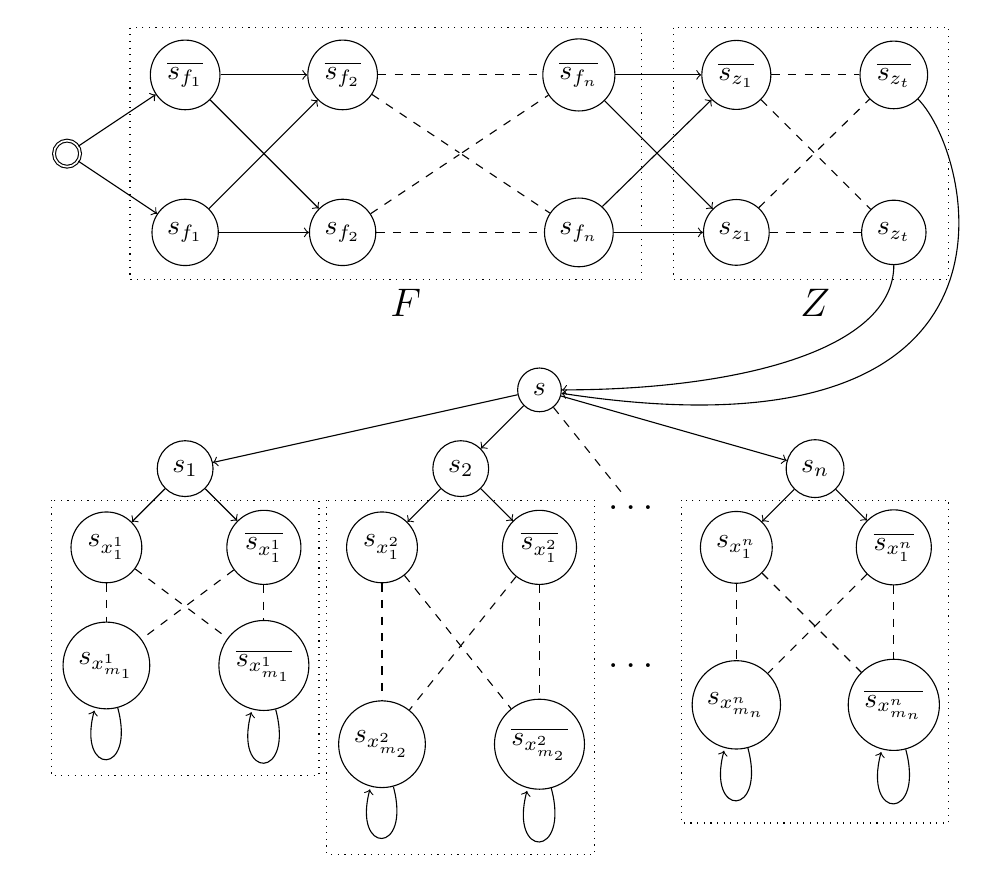
\begin{tikzpicture}

\path [use as bounding box] (-6.5,1.1) rectangle (5.5,-9.4);

\node [draw,double,circle] (v1) at (-6,-0.5) {$\sinit$};
\node [draw,circle] (v2) at (-4.5,-1.5) {$s_{f_1}$};
\node [draw,circle] (v3) at (-4.5,0.5) {$\overline{s_{f_1}}$};
\node [draw,circle] (v4) at (-2.5,-1.5) {$s_{f_2}$};
\node [draw,circle] (v5) at (-2.5,0.5) {$\overline{s_{f_2}}$};
\node [draw,circle] (v6) at (0.5,-1.5) {$s_{f_n}$};
\node [draw,circle] (v8) at (0.5,0.5) {$\overline{s_{f_n}}$};
\node [draw,circle] (v7) at (2.5,-1.5) {$s_{z_1}$};
\node [draw,circle] (v9) at (2.5,0.5) {$\overline{s_{z_1}}$};
\node [draw,circle] (v10) at (4.5,-1.5) {$s_{z_t}$};
\node [draw,circle] (v12) at (4.5,0.5) {$\overline{s_{z_t}}$};
\node [draw,circle] (v11) at (0,-3.5) {$s$};

\draw [->] (v1) edge (v2);
\draw [->] (v1) edge (v3);
\draw [->] (v2) edge (v4);
\draw [->] (v2) edge (v5);
\draw [->] (v3) edge (v4);
\draw [->] (v3) edge (v5);
\draw [->] (v6) edge (v7);
\draw [->] (v8) edge (v9);
\draw [->] (v6) edge (v9);
\draw [->] (v8) edge (v7);
\draw [dotted] (-5.2,1.1) rectangle (1.3,-2.1);
\draw [dotted] (1.7,1.1) rectangle (5.2,-2.1);


\node [inner sep=0, outer sep=0] (v15) at (-1,0.5) {};
\node [inner sep=0, outer sep=0] (v14) at (-1,-0.5) {};
\node [inner sep=0, outer sep=0] (v13) at (-1,-1.5) {};
\draw [dashed] (v4) edge (v13);
\draw [dashed] (v13) edge (v6);
\draw [dashed] (v4) edge (v14);
\draw [dashed] (v14) edge (v6);
\draw [dashed] (v5) edge (v14);
\draw [dashed] (v14) edge (v8);
\draw [dashed] (v5) edge (v15);
\draw [dashed] (v15) edge (v8);
\draw [dashed] (v7) edge (v10);
\draw [dashed] (v7) edge (v12);
\draw [dashed] (v9) edge (v10);
\draw [dashed] (v9) edge (v12);
\node at (3.5,-2.4) {\Large $Z$};
\node at (-1.7,-2.4) {\Large $F$};


\node [draw,circle] (v16) at (-4.5,-4.5) {$s_1$};
\node [draw,circle] (v17) at (-1,-4.5) {$s_2$};
\node [draw,circle] (v18) at (3.5,-4.5) {$s_n$};
\node [draw,circle] (v19) at (-5.5,-5.5) {$s_{x^1_1}$};
\node [draw,circle] (v20) at (-3.5,-5.5) {$\overline{s_{x^1_1}}$};
\node [draw,circle] (v21) at (-2,-5.5) {$s_{x^2_1}$};
\node [draw,circle] (v22) at (0,-5.5) {$\overline{s_{x^2_1}}$};
\node [draw,circle] (v23) at (2.5,-5.5) {$s_{x^n_1}$};
\node [draw,circle] (v24) at (4.5,-5.5) {$\overline{s_{x^n_1}}$};
\node [draw,circle] (v25) at (-5.5,-7) {$s_{x^1_{m_1}}$};
\node [draw,circle] (v26) at (-3.5,-7) {$\overline{s_{x^1_{m_1}}}$};
\node [draw,circle] (v27) at (-2,-8) {$s_{x^2_{m_2}}$};
\node [draw,circle] (v28) at (0,-8) {$\overline{s_{x^2_{m_2}}}$};
\node [draw,circle] (v29) at (2.5,-7.5) {$s_{x^n_{m_n}}$};
\node [draw,circle] (v30) at (4.5,-7.5) {$\overline{s_{x^n_{m_n}}}$};
\draw [->] (v11) edge (v16);
\draw [->] (v11) edge (v17);
\draw [->] (v11) edge (v18);
\node (v31) at (1.2,-5) {\Large \dots};
\node at (1.2,-7) {\Large \dots};
\draw [->] (v16) edge (v19);
\draw [->] (v16) edge (v20);
\draw [->] (v17) edge (v21);
\draw [->] (v17) edge (v22);
\draw [->] (v18) edge (v23);
\draw [->] (v18) edge (v24);
\draw [->] (v25) edge[loop below] (v25);
\draw [->] (v26) edge[loop below] (v26);
\draw [->] (v27) edge[loop below] (v27);
\draw [->] (v28) edge[loop below] (v28);
\draw [->] (v29) edge[loop below] (v29);
\draw [->] (v30) edge[loop below] (v30);
\draw [dashed] (v19) edge (v25);
\draw [dashed] (v19) edge (v26);
\draw [dashed] (v20) edge (v25);
\draw [dashed] (v20) edge (v26);
\draw [dashed] (v21) edge (v27);
\draw [dashed] (v21) edge (v28);
\draw [dashed] (v22) edge (v27);
\draw [dashed] (v22) edge (v28);
\draw [dashed] (v23) edge (v29);
\draw [dashed] (v23) edge (v30);
\draw [dashed] (v24) edge (v29);
\draw [dashed] (v24) edge (v30);
\draw [dashed] (v11) edge (v31);
\draw [dotted] (-6.2,-4.9) rectangle (-2.8,-8.4);
\draw [dotted] (-2.7,-4.9) rectangle (0.7,-9.4);
\draw [dotted] (1.8,-4.9) rectangle (5.2,-9);

\draw [->](v12) .. controls (5.5,-0.5) and (6.5,-4.5) .. (v11);
\draw [->](v10) .. controls (4.5,-3) and (2.5,-3.5) .. (v11);
\end{tikzpicture}}
%\vspace*{-0.5cm}
\caption{The Kripke structure $\mathpzc{K}_{PAR}^{\Gamma}$.}\label{Kpar}
\end{figure}
%
$\mathpzc{K}_{PAR}^{\Gamma}$ features a pair of states for each Boolean variable in $F\cup Z$ as well as for all the variables of formulas in $\Gamma$ (one state for each truth value). Each path from the initial state $\sinit$ to the state $s$ represents a truth assignment to the variables in $F \cup Z$. Then, the structure branches into $n$ substructures, each one modeling 
the possible truth assignments to the variables of a formula in $\Gamma$. 

Formally, $\mathpzc{K}_{PAR}^{\Gamma}=\KuDef$, where
\begin{itemize}
    \item $\Prop=\{p,q\}\cup F \cup Z \cup \{aux_i\mid 1\leq i\leq n\}\cup \{x^i_{j_i}\mid 1\leq i\leq n,\; 1\leq j_i\leq m_i\}$,
    \item $\States=\{\sinit\}\cup\{s_{f_i}, \overline{s_{f_i}}\mid 1\leq i\leq n\}\cup\{s_z,\overline{s_z} \mid z\in Z\}\cup\{s\}\cup\{s_i\mid 1\leq i\leq n\}\cup $ \\
    $\{s_{x^i_{j_i}}, \overline{s_{x^i_{j_i}}}\mid 1\leq i\leq n,\; 1\leq j_i\leq m_i\}$,
    \item $\Edges\!=\!\{(\sinit,s_{f_1}),(\sinit,\overline{s_{f_1}})\}\cup \{(s_{f_i},s_{f_{i+1}}),(s_{f_i},\overline{s_{f_{i+1}}}),(\overline{s_{f_i}},s_{f_{i+1}}),(\overline{s_{f_i}},\overline{s_{f_{i+1}}})\mid 1\!\leq\! i\!<\! n\} \cup$\\
    $\{(s_{f_n},s_{z_1}),(\overline{s_{f_n}},s_{z_1}),(s_{f_n},\overline{s_{z_1}}),(\overline{s_{f_n}},\overline{s_{z_1}})\}\cup$\\
    $\{(s_{z_i},s_{z_{i+1}}),(s_{z_i},\overline{s_{z_{i+1}}}),(\overline{s_{z_i}},s_{z_{i+1}}),(\overline{s_{z_i}},\overline{s_{z_{i+1}}})| 1\leq i< t\} \cup$\\
    $\{(s_{z_t},s),(\overline{s_{z_t}},s)\}\cup \{(s,s_i),(s_i,s_{x^i_1}),(s_i,\overline{s_{x^i_1}})\mid 1\leq i\leq n\}\cup$ \\
    $\{(s_{x^i_{j_i}},s_{x^i_{j_i+1}}), (\overline{s_{x^i_{j_i}}},s_{x^i_{j_i+1}}),(\overline{s_{x^i_{j_i}}},s_{x^i_{j_i+1}}),(\overline{s_{x^i_{j_i}}},\overline{s_{x^i_{j_i+1}}}) | 1\leq i\leq n,\; 1\leq j_i< m_i\}\cup$\\
    $\{(s_{x^i_{m_i}},s_{x^i_{m_i}}),(\overline{s_{x^i_{m_i}}},\overline{s_{x^i_{m_i}}})|1\leq i\leq n\}$,
    \item and the labeling function $\Lab$ is defined as follows:
	\begin{itemize}
		\item $\Lab(\sinit)=\{p,q\}\cup F\cup Z$;
		\item for all $1\leq i\leq n$, $\Lab(s_{f_i})=\{p,q\}\cup F\cup Z$; $\Lab(\overline{s_{f_i}})=\{p,q\}\cup (F\setminus \{f_i\}) \cup Z$;
		\item for all $z\in Z$, $\Lab(s_z)=\{p,q\}\cup F\cup Z$; $\Lab(\overline{s_z})=\{p,q\}\cup F \cup (Z\setminus \{z\})$;
		\item $\Lab(s)=\{q\}\cup F\cup Z \cup \{aux_i\mid 1\leq i\leq n\}\cup \{x^i_{j_i}\mid 1\leq i\leq n,\; 1\leq j_i\leq m_i\}$;
		\item for all $1\leq i\leq n$, $\Lab(s_i)= \{aux_i\}\cup \{x^i_{j_i}\mid 1\leq j_i\leq m_i\}$;
		\item for all $1\leq i\leq n$, $1\leq k_i\leq m_i$, $\Lab(s_{x^i_{k_i}})= \{aux_i\}\cup \{x^i_{j_i}\mid 1\leq j_i\leq m_i\}$;  $\Lab(\overline{s_{x^i_{k_i}}})= \{aux_i\}\cup \{x^i_{j_i}\mid 1\leq j_i\leq m_i\}\setminus\{x^i_{k_i}\}$.
	\end{itemize}
\end{itemize}
%  
According to the definition of $\mathpzc{K}_{PAR}^{\Gamma}$, it holds that:
\begin{enumerate}
\item each trace $\rho$ from $\sinit$ to $s$ encodes a truth assignment to the proposition letters in $F\cup Z$ (for all $y\in F\cup Z$, $y$ is $\top$ in $\rho$ if and only if $y\in\bigcap_{w\in\states(\rho)}\Lab(w)$). Conversely, for each truth assignment to the proposition letters in $F\cup Z$, there exists an initial trace $\rho$, reaching the state $s$, encoding such an assignment. Note that, among the initial traces, the ones leading to $s$ are exactly those satisfying $q \wedge \neg p$.
%
\item An initial trace leading to $s$ satisfies $\text{parity}(F, Z)$ if the induced assignment sets an even number of $f_i$'s to $\top$, and every $z\in Z$ to the truth value which is functionally implied by the values of the $f_i$'s.
%
\item A trace $\tilde{\rho}$ starting from $s$ and ending in a state $s$, $s_i$, $s_{x_j^i}$ or $\overline{s_{x_j^i}}$, with $1 \leq i \leq n$ and $1 \leq j \leq m_i$, encodes a truth assignment to the proposition letters $x_1, \ldots, x_{m_i}$ (if the trace 
ends in $s$ or $s_i$, all the variables are assigned to $\top$; if it ends in $s_{x_j^i}$ or $\overline{s_{x_j^i}}$, in particular all the variables 
$x^i_{j+1}, \ldots , x^i_{m_i}$ are assigned to $\top$, by homogeneity).
%
\item A Boolean formula $\phi_i(x_1^i,\ldots , x_{m_i}^i) \in \Gamma$ is satisfiable if and only if there exists a trace $\tilde{\rho}$ starting from $s$ and ending in a state $s$, $s_i$, $s_{x_j^i}$ or $\overline{s_{x_j^i}}$, for some $j=1,\ldots , m_i$, such that $\mathpzc{K}_{PAR}^{\Gamma},\tilde{\rho}\models \phi_i(x_1^i,\ldots , x_{m_i}^i)$. 
\end{enumerate}

Finally, let us consider the $\A$ formula 
\[\psi=q \wedge \neg p \wedge \text{parity}(F, Z) \wedge \bigwedge_{i=1}^n \big(f_i \leftrightarrow \hsA(aux_i \wedge \phi_i(x_1^i,\ldots , x_{m_i}^i))\big).\]
%
In view of the above observations, $\psi$ is satisfied by an initial trace $\overline{\rho}$ if (and only if) $(i)$ $\overline{\rho}$ leads to $s$, $(ii)$ $\overline{\rho}$ induces an assignment which sets an even number of $f_i$'s to $\top$ and all $z\in Z$ accordingly, and $(iii)$
%Moreover, the conjunct $\bigwedge_{i=1}^n \big(f_i \leftrightarrow \hsA(aux_i \wedge \phi_i(x_1^i,\cdots , %x_{m_i}^i))\big)$ is satisfied by $\overline{\rho}$ when, 
for all $1 \leq i \leq n$, $f_i$ is $\top$ if and only if there exists a trace $\tilde{\rho}$ starting from $s$ and ending in a state $s$, $s_i$, $s_{x_j^i}$ or $\overline{s_{x_j^i}}$, such that $\mathpzc{K}_{PAR}^{\Gamma},\tilde{\rho}\models \phi_i(x_1^i,\ldots , x_{m_i}^i)$.
The length of $\psi$ is polynomial in the input size.

Let us now assume we are given an instance of PARITY(SAT) $\Gamma$ with an \emph{even} number of satisfiable Boolean formulas. Then, there exists an initial trace $\rho$ ending in $s$ such that, for all $i$, $s_{f_i}\in\states(\rho)$ if $\phi_i(x_1^i,\ldots , x_{m_i}^i)$ is satisfiable, and $\overline{s_{f_i}}\in\states(\rho)$ otherwise. Moreover, $\rho$ can be chosen in such a way that $\mathpzc{K}_{PAR}^{\Gamma},\rho\models  \text{parity}(F,Z)$. It immediately follows that, for all $i$, $\mathpzc{K}_{PAR}^{\Gamma},\rho\models f_i$ if and only if $\mathpzc{K}_{PAR}^{\Gamma},\rho\models \hsA(aux_i \wedge \phi_i(x_1^i,\ldots , x_{m_i}^i))$, concluding that $\mathpzc{K}_{PAR}^{\Gamma},\rho\models \psi$.

Conversely, let $\rho$ be  an initial trace such that $\mathpzc{K}_{PAR}^{\Gamma},\rho\models \psi$. It holds that 
$\rho$ ends in $s$ and sets an even number of $f_i$'s to $\top$. Furthermore, if $\mathpzc{K}_{PAR}^{\Gamma},\rho\models f_i$, then there exists $\tilde{\rho}$ starting from $s$ and ending in $s$, $s_i$, $s_{x_j^i}$ or $\overline{s_{x_j^i}}$, such that $\mathpzc{K}_{PAR}^{\Gamma},\tilde{\rho}\models\phi_i(x_1^i,\ldots , x_{m_i}^i)$, hence $\phi_i(x_1^i,\ldots , x_{m_i}^i)$ is satisfiable.
If $\mathpzc{K}_{PAR}^{\Gamma},\rho\models \neg f_i$, then there exists no $\tilde{\rho}$ starting from $s$ and ending in $s$, $s_i$, $s_{x_j^i}$ or $\overline{s_{x_j^i}}$, such that $\mathpzc{K}_{PAR}^{\Gamma},\tilde{\rho}\models\phi_i(x_1^i,\ldots , x_{m_i}^i)$. Thus $\phi_i(x_1^i,\ldots , x_{m_i}^i)$ is unsatisfiable. Hence, $\Gamma$ contains an even number of satisfiable formulas.

Therefore we have proved that the number of \emph{satisfiable} Boolean formulas of $\Gamma$ is \emph{even} if and only if there exists an initial trace $\rho$ such that $\mathpzc{K}_{PAR}^{\Gamma},\rho\models \psi$. 
%Equivalently, 
This amounts to say that $\Gamma$ contains an \emph{odd} number of satisfiable Boolean formulas (the PARITY(SAT) problem) if and only if $\mathpzc{K}_{PAR}^{\Gamma}\models \Phi_{\Gamma}$, where $\Phi_{\Gamma}=\neg\psi$ (the MC problem).
The next theorem immediately follows.
\begin{theorem}
The MC problem for $\A$ formulas over finite Kripke structures is $\Th$-hard (under polynomial-time reductions).
\end{theorem}

A similar proof can be given for $\Abar$ (roughly speaking, we replace all the occurrences of $\hsA$ in $\Phi_{\Gamma}$ by $\hsAt$, and we stick the $n$ substructures of $\mathpzc{K}_{PAR}^{\Gamma}$---after transposing all their edges---on $\sinit$, instead of $s$).

Finally, we observe that the $\Th$-hardness of $\Abar$ and $\A$ immediately propagates to $\AAbar$, $\AbarB$ and $\AE$, yielding, together with Corollary~\ref{th:AAbaralgo} and Theorem~\ref{th:AbarBalgo}, the following result.
%
\begin{theorem}
The MC problem for $\A$, $\Abar$, $\AAbar$, $\AbarB$ and $\AE$ formulas over finite Kripke structures is in $\Thsq$ and it is hard for $\Th$.
\end{theorem}

It is still an open issue if MC for the above fragments can be solved by $o(\log^2 n)$ queries to the $\NP$ oracle, or it is possible to prove a stronger lower bound, or both (e.g., the problem may be complete for $\PTIME^{\NP[O(\log n \log\log n)]}$). As a matter of fact, any attempt to reduce \TBSATM{} \emph{to} MC for $\A$, $\AE$, or $\AAbar$ has failed, because in such \lq\lq reduction\rq\rq{} we need an $\HS$ formula of length $\Theta(n^{\log n})$, which clearly cannot be generated in polynomial time.